\documentclass[a4paper,12pt]{scrreprt}
\usepackage[T1]{fontenc}
\usepackage[utf8]{inputenc}
\usepackage[ngerman]{babel}
\usepackage[table]{xcolor}% http://ctan.org/pkg/xcolor
\usepackage{tabu}
\usepackage{graphicx}



\begin{document}


\author{Dominik Backhausen \and Daniel Dimitrijevic \and Alexander Rieppel \and Thomas Traxler}
\subject{Pflichtenheft}
\title{LAN Yourself}
\date{\today}
\maketitle
\tableofcontents

\chapter{Projekt-Team}
	\begin{itemize}
	\item Dominik Backhausen\\
	F"ahigkeiten:Java, Html, C/C++, SQL
	\item Daniel Dimitrijevic\\
	F"ahigkeiten: Java, Html,C/C++, SQL
	\item Alexander Rieppel\\
		F"ahigkeiten:Java, Html, C/C++, SQL    
	\item Thomas Traxler\\
	F"ahigkeiten:Java, XML, C/C++, SQL
	\end{itemize}
	
	
\chapter{Zielbestimmung}
	\begin{itemize}
	\item Peer-to-Peer Prinzip (gegebenenfalls Hybrid)
	\item Erstellung von VANs
	\item intuitives GUI-Design
	\item Konfigurationsdateien f"ur erweiterte Einstellungen
	\item Netzwerkteilnehmerliste
	\item Senden von Textnachrichten
	\end{itemize}
	
	\section{Zul"assige Erweiterungen}
	
	\begin{itemize}
				\item Weiterleitung der Internetverbindung
				\item Einstellung ob die Internetverbindung des LAN-Netzwerks oder die eigene verwendet werden soll
				\item Zugriffspunkt f"ur die Internetverbindung im VAN nach bestimmten Kriterien aussuchen lassen, wobei dies entweder manuell oder "uber einen Algorithmus erfolgen kann
				
				\item Ports am Internetzugriffspunkt zu bestimmten Netzwerkteilnehmern weiterleiten
				\item Gemeinsame Ordner erstellen und bestimmten Netzwerkteilnehmern freigeben
				
				\item Onion-Routing (Pfadauswahl auch durch Kriterien m"oglich)
				
				\end{itemize}
	
	\section{Unzul"assige Erweiterungen / Nichtziele}
	
	\begin{itemize}
	\item Es ist kein Ziel die Software nach ihrer Fertigstellung zu vermarkten
	\item Es ist kein Ziel auf einer eigens programmierten VPN-Basis aufzusetzen
	
	\end{itemize}
	
	
\chapter{Produkteinsatz}
	
	\section{Anwendungsbereiche}
	 Die Software ist in erster Linie f"ur Firmen gedacht die ein schnelles und einfaches VPN-Netzwerk ben"otigen. Dabei ist wichtig, dass verschiedenste Varianten dieses Szenarios denkbar sind, wie z.B. Mitarbeiter die international, auf allen Kontinenten verteilt, miteinander sicher kommunizieren m"ussen und gleichzeitig, im selben Netzwerk, Zugriff auf die internen Dienste der Firma ben"otigen (Server, Datenbank, etc.). Da die Software auch daf"ur ausgelegt ist, mit m"oglichst vielen verschiedenen Programmen zu funktionieren, sind die Anwendungsbereiche vielf"altig. Deshalb ist sie nicht nur f"ur Firmen, sondern auch f"ur Privatpersonen interessant die ein VPN-Netzwerk einrichten, dabei m"oglichst flexibel und benutzerfreundlich bleiben wollen, aber sich die komplizierte Einrichtung eines VPN-Servers ersparen m"ochten.

	\section{Zielgruppe}
	
	Generell kann man die Zielgruppe auf die folgenden gro"se Gruppen einschr"anken:
	\begin{itemize}
	\item Mitarbeiter die sich per VPN mit dem Intranet der Firma verbinden, um auf interne Server zuzugreifen und gleichzeitig m"oglichst sicher und international miteinander verbunden sein wollen
	\item Private Personen mit dem Wunsch eines VPN-Netzwerks
	\end{itemize}
		
	\section{Betriebsbedingungen}
	Damit diese Software lauff"ahig ist, wird ein PC mit zumindest Microsoft Windows XP und einer funktionierenden Netzwerkkarte, die eine Verbindung mit dem Internet herstellen kann, ben"otigt. Auch wird die aktuellste Version der VPN-Basis ben"otigt, welche bereits in der Auslieferungsversion der Software enthalten ist.
		
\chapter{Produktumgebung}
	
	\section{Software}
		
		Unsere Software ben"otigt die aktuellste Version der VPN Basis, welche mit unserem Produkt gleich mit ausgeliefert wird. Des weiteren wird die Funktionalit"at vorerst nur unter Windows 7 garantiert, eine Erweiterung der Kompatibilit"at unserer Software in diesem Punkt ist angedacht. Demnach steht eine Erweiterung der garantierten Funktionalit"at auf dem Plan, jedoch nicht als Teil dieses Projektes.
		
	\section{Hardware}
		
		Das Produkt wir ann"ahernd die selben Anforderungen an die Hardware haben wie die VPN Basis, dies entspricht ann"ahernd jedem handels"ublichen, Windows-kompatiblen Computer.	
		
	\section{Produktschnittstellen}
		
		Die Hauptschnittstelle des Produkts ist die VPN Basis, da diese f"ur jegliche Kommunikation verwendet wird. 
		
\chapter{Produktfunktionen}
		\section{Festlegen der Hauptfunktionen}
			\textbf{/HF10/ Verbinden mit einem VAN bzw. VAN erstellen}
					
					Jeder Benutzer muss sich mittels eines Benutzernamens erkennbar machen, Identifikation erfolgt jedoch mittels anderer Parameter (IP und Host-File). \\
					
					
					\textbf {/HF20/ Netzwerkteilnehmer anzeigen
					}\\
					Umfasst die Anzeige von:
					
					\begin{itemize}
					\item Latenzzeit
					\item IP-Adresse
					\item Benutzername
					\item Zugriffspunkt (ja/nein) \footnote{Kannziel}\\
					\end{itemize}
					
					
					
					
					
					\textbf {/HF30/ Textnachrichten an Netzwerkteilnehmer senden}
					\\Auch eine Kommunikation "uber Textnachrichten unter den Teilnehmern wird m"oglich sein.
					
					 \textbf {/HF40/ Konfigurationsdateien f"ur erweiterte Einstellungen}
					\\Dadurch wird erfahrenen Benutzern die M"oglichkeit gegeben erweiterte Einstellungen, die in der VPN-Basis verf"ugbar sind, zu verwenden.
			
		\section{Festlegung der Nebenfunktionen}
		\textbf { /NF10/ Internetverbindung im VAN freigeben} 
			\\Ein Teil oder der gesamte Internettraffic (falls nur ein Teilnehmer seine Internetverbindung freigegeben hat), den andere Teilnehmer produzieren, wird "uber diese Verbindung geroutet.
					
			\textbf {/NF20/ Mit dem Internet verbinden} 
			\\Der Benutzer kann festlegen ob er standardm"a"sig seine eigene Internetverbindung oder "uber einen Zugriffspunkt\footnote{Der Zugriffspunkt ist hier ein User der zur Verbindung mit dem Internet dient, d.h. seine Internetverbindung freigegeben hat} in seinem VAN ins Internet gehen m"ochte.
			
			\textbf {/NF30/ Netzwerkteilnehmer f"ur Internetverbindung nach Kriterien ausw"ahlen lassen}
			
			\textbf {/NF31/ Netzwerkteilnehmer f"ur Internetverbindung manuell ausw"ahlen}
			\\Es soll m"oglich sein einen bestimmten Netzwerkteilnehmer, aus dem Pool der Teilnehmer die ihre Verbindung freigegeben haben auszuw"ahlen, um "uber diesen Teilnehmer eine Internetverbindung aufzubauen.
			
			\textbf {/NF32/ Netzwerkteilnehmer f"ur Internetverbindung nach Algorithmus bestimmen}
			\\Ebenfalls soll es m"oglich sein den optimalen Netzwerkteilnehmer automatisch nach einem bestimmten Kriterium (Latenzzeit, zur Verf"ugung stehende Bandbreite, etc.) ausw"ahlen zu lassen.
			
			\textbf {/NF40/ Gemeinsamen Ordner erstellen}
			\\Eine weitere Funktion ist das Erstellen eines gemeinsamen Ordners, der innerhalb des Netzwerks freigegeben werden kann. Zus"atzlich wird es m"oglich sein Berechtigungen f"ur diesen Ordner festzulegen und die Benutzer auszuw"ahlen, die auf ihn zugreifen d"urfen.
			
			\textbf {/NF50/ Netzwerkteilnehmer ignorieren}
			\\Ein Netzwerkteilnehmer kann andere Netzwerkteilnehmer von der Software ignorieren lassen. Dies bedeutet, dass die Kommunikation "uber das Netzwerk zwischen diesen Teilnehmern nicht l"anger m"oglich ist solange diese Sperre besteht.
		
\chapter{Produktdaten}
	
	\section{Festlegen der Hauptdaten}
				\textbf {/HD10/ Benutzername}
				
				Verwendeter Benutzername\\
				\textbf {/HD20/ Gespeicherte Daten der anderen Netzwerkteilnehmer}
				
				Daten wie IP-Adresse oder Ports die f"ur die Verbindung verwendet werden sollen\\
				\textbf {/HD30/ Einstellungen}
				
				Vorgenommene Einstellungen in der Software\\

\chapter{Produktleistungen}
	\textbf{/LL10/ Optimierter Datenverkehr durch Peer-to-Peer}
			
			Da hier keine Server-Client Architektur verwendet wird, ist auch der Datenverkehr, der "uber einen einzigen Netzwerkteilnehmer gef"uhrt wird, deutlich geringer.\\
			\textbf {/LL20/ Hohe Erweiterbarkeit der Software}
			
			Das Endprodukt soll die Bedingungen der einfachen Wartbarkeit und Erweiterbarkeit erf"ullen. Dies bedeutet das Softwarecode sowohl verst"andlich geschrieben als auch gut dokumentiert ist, au"serdem werden die Programmteile einer klaren Aufteilung unterliegen.\\
			\textbf {/LL30/ Hohe Kompatibilit"at zu verschiedenen Programmen}
			
			Bei der Entwicklung der Software wird besonders darauf geachtet, dass sie mit verschiedenen Programmen kompatibel ist.\\
			\textbf {/LL40/ Hohe Performanz}
			
			Hiermit ist sowohl Performanz innerhalb des Programms, als auch im Netzwerk gemeint.
	
	
	
	
\chapter{Benutzerschnittstelle}
Bestehende Programme haben oft eine unzureichend intuitive oder nicht ausreichend erkl"arte Benutzeroberfl"ache, in denen sich unerfahrene Benutzer nur sehr schwer zurechtfinden. Deshalb wird das Programm besonders intuitiv und simpel verwendbar sein. Es wird dar"uber hinaus ein kleines Hilfemen"u geben um Einsteigern die Benutzung noch einfacher zu gestalten.
	
	
\chapter{Qualit"atsbestimmungen}
\section{Sicherheit}
	Das Produkt wird stark auf den Einsatz durch viele Benutzer zugeschnitten. Um in dieser Gemeinschaft dem Abh"oren von "ubertragenen Daten durch Au"senstehende vorzubeugen, werden alle Daten verschl"usselt.
		 
	\section{Benutzbarkeit}
	Bei der Entwicklung wird "au"serst viel Wert auf eine intuitive und einfache GUI gelegt, die sowohl die Performanz als auch das Design betreffend, die erw"unschten Ergebnisse liefert und damit dem Benutzer zugute kommt, anstatt lediglich ein notwendiges "Ubel darzustellen. 
			
	\section{Effizienz}
	Da bei unserem Programm  mit vielen Benutzern gerechnet wird und diese auch viele Daten verschicken, muss unser Programm imstande sein eine durchgehende und stabile Verbindung zu unterst"utzen. Dies bedeutet in erster Linie die notwendigen Neukonfigurationen an der VPN-Basis zu optimieren. Weiters ist es notwendig, dass die Software zeitkritische Aktionen priorisiert und daher schnell und effizient abarbeitet.
		
		
	\section{Erweiterbarkeit}
	Wie bereits bei den Hauptleistungen erw"ahnt, ist vorgesehen das Programm so zu schreiben, dass zuk"unftige Erweiterungen der Software leicht m"oglich sind. 
		
	\section{"Ubertragbarkeit}
	Da entschieden wurde das Programm f"ur Windows zu optimieren, wird in weiterer Hinsicht weniger Wert auf die "Ubertragbarkeit der Software zu anderen Betriebssystemen gelegt. Dennoch wird es m"oglich sein (durch Zutun des Benutzers) eigene Versionen zu erstellen, die in weiterer Folge auch auf Linux oder Mac OSX lauff"ahig sind.
%\chapter{Globale Testf"alle}
%
%	\begin{figure}[h]
%		\centering
%		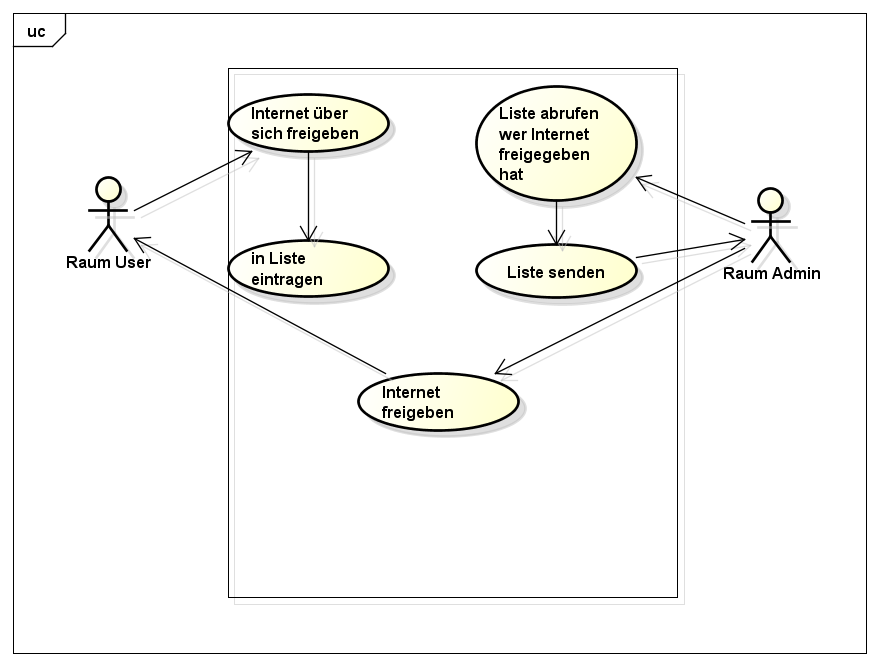
\includegraphics[width=0.9\linewidth]{VPN_Internet_freigeben}
%		\caption{}
%		\label{fig:VPN_Internet_freigeben}
%	\end{figure}
%	\begin{figure}[h]
%		\centering
%		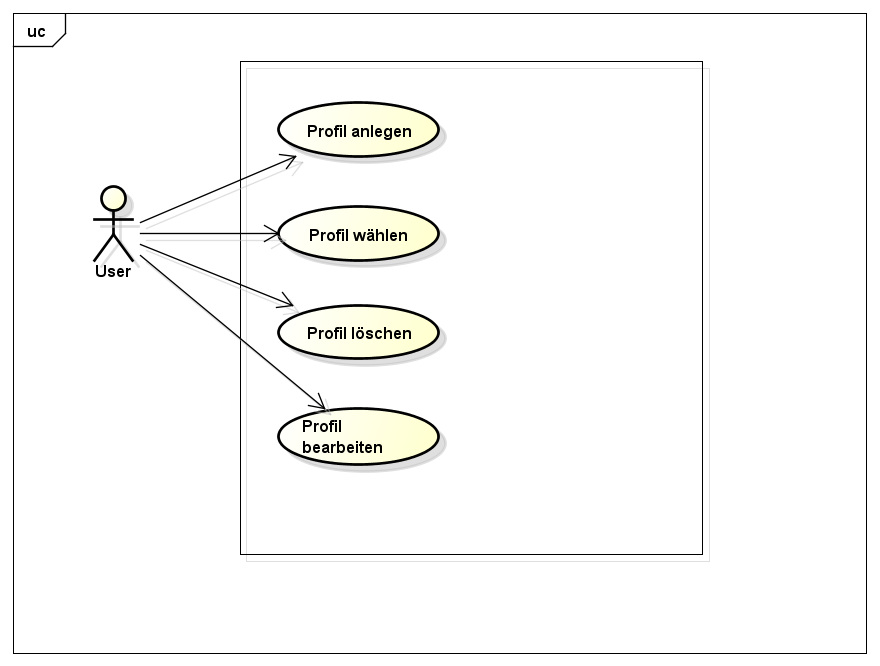
\includegraphics[width=0.9\linewidth]{VPN_Profilemanager}
%		\caption{}
%		\label{fig:VPN_Profilemanager}
%		\end{figure}
%	\begin{figure}[h]
%		\centering
%		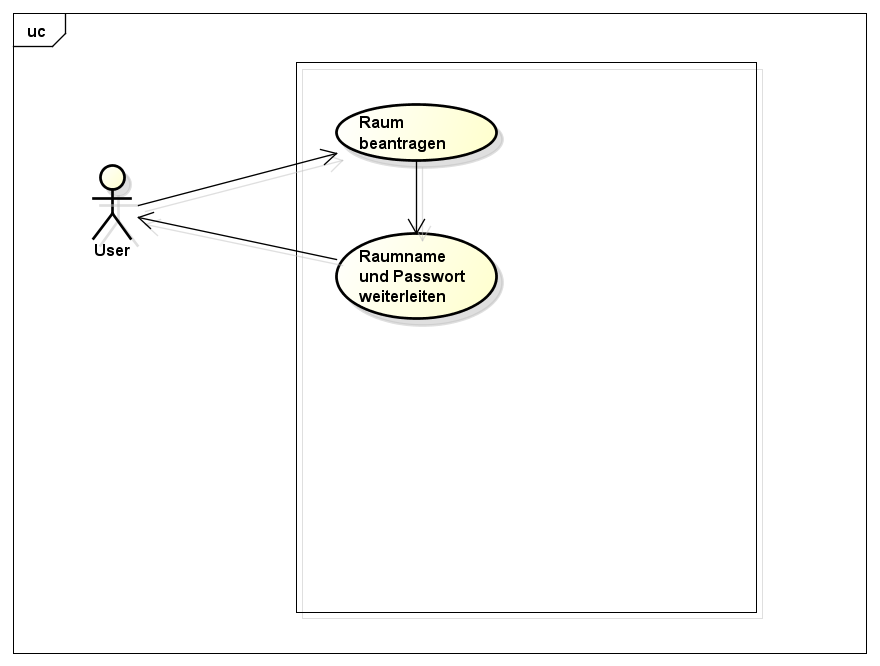
\includegraphics[width=0.9\linewidth]{VPN_Raum_Beantragen}
%		\caption{}
%		\label{fig:VPN_Raum_Beantragen}
%	\end{figure}
%	\begin{figure}[h]
%		\centering
%		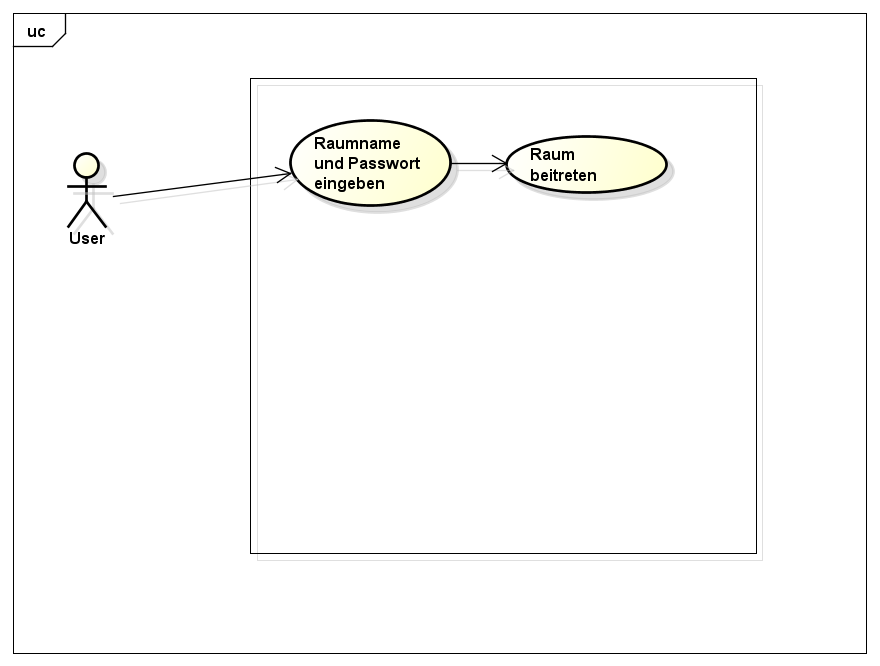
\includegraphics[width=0.9\linewidth]{VPN_Raum_Beitreten}
%		\caption{}
%		\label{fig:VPN_Raum_Beitreten}
%	\end{figure}

	
\chapter{Entwicklungsumgebung}
	
	\section{Software}
		Zur Entwicklung der Software wird jeder seine Entwicklungsumgebung benutzen d"urfen. Falls es zu Fehlern zwischen denn Entwicklungsumgebungen kommt werden wir uns auf eine einigen und nur mit dieser weiter arbeiten. 
		
		Eclipse: Wird als Hauptentwicklungsumgebung benutzt werden da alle Mitarbeiter bisher haupts"achlich in dieser mit Java gearbeitet haben.
		
	\section{Hardware}
		
		Die Software wird auf PCs mit Microsoft Windows 7 und einer lauff"ahigen Netzwerkkarte entwickelt.
	
\end{document}